\subsection{21. Линейные и полулинейные множества. Теорема Парика: полулинейность КС-языков.}

\textbf{Лемма:} $\forall X \subseteq \mathbb{N}^{|\Sigma|}$ полулинейного $\exists$ R (полулинейный) - регулярный язык ($\psi(R) = X$)

\textbf{Теорема Па'рика:} L - КС язык $\Rightarrow$ L - полулинейный.

Введём \textbf{лемму о разрастании}: G - КС язык. Тогда: $\forall k \exists p: \forall w \in L$ : $|w| \geqslant p$ $\exists w = xu_1\dots u_kyv_k \dots v_2v_1z$: $|u_iv_i| > 0, |u_1 \dots u_kyv_k \dots v_1| \leqslant p$

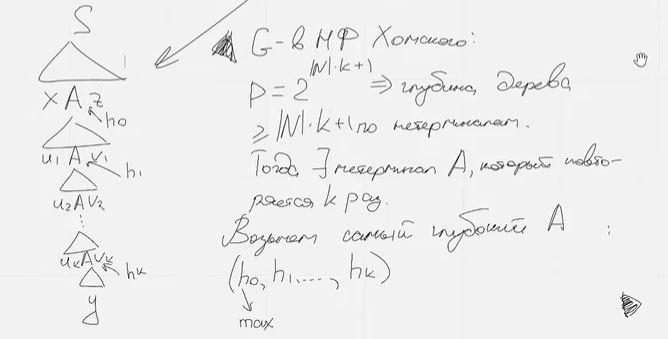
\includegraphics[]{images/parikh3.JPG}

$\blacktriangle$ G - в НФ Хомского, $p = 2^{|N|k + 1}$ $\Rightarrow$ глубина дерева $\geqslant |N|k + 1$ по нетерминалам. Тогда $\exists$ нетерминал А, который повторяется k раз. Возьмём самый глубокий А: $(h_0, h_1, \dots, h_k)$
$\blacksquare$

Док-во теоремы Парика:

$\blacktriangle$ $L = L(G)$: G - в НФ Хомского, $= <N, \Sigma, P, S>$. $\forall M \subset N: L_M(G) = \{w|S \vdash w$ при помощи только нетерминалов из M, причём всех $\}$.

Надо доказать, что $L_M(G)$ - полулинейно (тогда $L(G)$ - объединение конечного числа полулинейных множеств и как следствие полулинейно). Возьмём p из леммы о разрастании, $k = |N|$. $X = \{ \psi(w) | w\in L_M(G), |w| \leqslant p\}$, $Y = \{ \psi(uv) | |uv| \leqslant p \&\& \exists B \vdash uBv$ из нетерминалов M $\}$

Лемма: $\psi(L_M(G)) = X + <Y>$.

$\Leftarrow$: $x \in X + <Y>$. $x = x_1 + \alpha_1y_1 + \dots + \alpha_m y_m$; $x_1 \in X \Rightarrow \exists w': w' \in L_M(G), |w'| \leqslant p$. 

$y_i \in Y \Rightarrow \exists w_i = u_iv_i:$ вывод $B_i \vdash u_iBv_i$ из M. Финт ушами: $w' \in L_M(G) \Rightarrow$ $\exists$ вывод со всеми нетерминлами B: рисуем ёлку вида

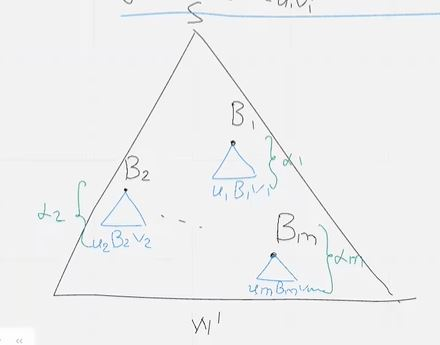
\includegraphics[]{images/new_year_tree.JPG}

w'' - слово после "подвешивания" $B_i \vdash u_iB_iv_i$ к дереву вывода; $w'' \in (L_M(G): \psi(w'') = x$

Победа!

$\Rightarrow$: $w \in L_M(G) \Rightarrow \psi(w) \in X + <Y>$.

Индукция по длине слова.

База: $|w| \leqslant p \Rightarrow \psi(w) \in X$.

Переход: для $k = |N|$ лемма о разрастании:

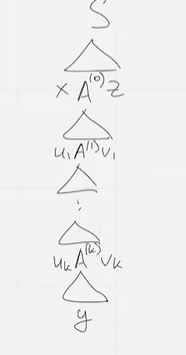
\includegraphics[width=2cm]{images/parikh4.JPG}

$M_i$ - множество нетерминалов, не считая А, которые встречаются в выводе: $A^{(i)} \vdash u_{i+1}u_{i+2} \dots u_k y v_k \dots v_{i+1}$. Тогда $|M| > |M_0| \geqslant |M_1| \geqslant |M_2| \geqslant \dots \geqslant |M_k| \geqslant 0$; k+1 число = $|N| + 1$ число от 0 до $|M| - 1$. Тогда по принципу Дирихле $\exists j: M_j = M_{j+1}$.

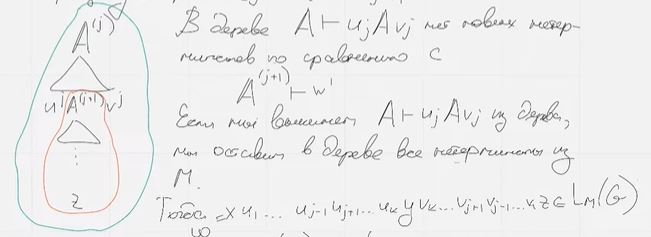
\includegraphics[]{images/parikh5.JPG}

$\psi(w) = \psi(\omega) + \psi(u_jv_j)$, $\psi(\omega) \in X + <Y>, \psi(u_jv_j) \in Y$ (первое по предположению индукции). Ура!

$\blacksquare$